\documentclass[11pt]{article}
\usepackage[utf8]{inputenc}
\usepackage[T1]{fontenc}
\usepackage{amsmath,amssymb,amsthm}
\usepackage{booktabs}
\usepackage{graphicx}
\usepackage{hyperref}
\usepackage{xcolor}
\usepackage{enumitem}
\usepackage[margin=1in]{geometry}
%\usepackage{multirow}
\usepackage{tabularx}
\usepackage{tikz}
\usepackage{caption}
\usepackage{subcaption}
\usepackage{float}
\usetikzlibrary{arrows.meta,positioning,shapes.geometric,fit,calc}

\hypersetup{
  colorlinks=true,
  linkcolor=blue!70!black,
  citecolor=blue!70!black,
  urlcolor=blue!70!black
}

\newcommand{\tbd}[1]{\textcolor{red}{\textbf{[TBD: #1]}}}
\newcommand{\arbiter}{\textsc{Arbiter}}

\title{Arbiter: From PDF to Verdict --- Formal Verification Stipulations\\for Multi-Agent Research Claim Debate}

\author{Vishnu Kchitti}

\date{April 2026}

\begin{document}
\maketitle

\begin{abstract}
Research papers routinely overreach beyond their evidence.
The replication crisis (36\% of landmark results replicate), tripling retraction rates, and growing skepticism toward LLM-as-judge evaluation demand tools that distinguish what a paper \emph{proves} from what it \emph{claims}.
We present \arbiter{}, an open-source framework (11K~LOC Python, 7~LLM providers) that implements a complete PDF-to-verdict pipeline: it reads academic papers with formal or quantitative claims, extracts those claims, attempts machine verification via Knuckledragger (Z3) and SymPy, stages multi-agent debates with argumentative validity enforcement, and produces verdicts from a multi-provider evaluation panel.
In an extended case study on \emph{The AI Layoff Trap} (Falk \& Tsoukalas, 2026), \arbiter{} assembled 9~specialist agents across 3~frontier providers (GPT-5.4, Claude Opus 4.6, Grok~4.20), which produced 141~substantive argument exchanges across 54~turns over 6~rounds (``argument hits'' counts distinct claims advanced or rebutted per turn, not correctness).
The debate surfaced 17~Proponent concessions (the Proponent agent argues for the paper's claims)---revealing that the paper's core theorem ($\alpha_{\mathrm{NE}} > \alpha_{\mathrm{CO}}$ when $\eta < 1, N > 1$) is mathematically correct, but its headline policy claims (``only a Pigouvian tax can fix over-automation'') extend far beyond the mathematics.
We replicate this pattern on two additional papers (model-collapse anti-Singularity; strict-safety/AGI impossibility), yielding 13~and 9~Proponent concessions respectively. Across all three (Section~\ref{sec:additional_casestudies}), formal theorems survive while policy/existential claims overreach in three distinct ways---policy exclusivity, scope generalization, definition mismatch---each flagged by the init-phase contradiction detector (e.g., C43 vs.\ C126; C5 vs.\ C29). N=3 single runs with no gold labels; the consistency is suggestive, not a statistical generalization.
A pilot ablation on the Layoff paper suggests debate with verification may elicit more concessions than debate alone or LLM-as-judge; N=1 for the ablation itself, so this is illustrative rather than conclusive.
As a byproduct of building the verification backend, we characterize failure modes in LLM-generated Z3 proofs and report certificate validity rates for our own pipeline; we find that Z3-based proof generation requires careful audit, as LLMs frequently produce encodings that are technically satisfiable but do not faithfully represent the mathematical claim.
We report these findings transparently; the verification backend is a work in progress, and honest measurement is a prerequisite to improvement.
Code and all experimental artifacts are available at \url{https://github.com/vishk23/arbiter}. All experiments were conducted in April 2026 using frontier models available at that time (GPT-5.4, Claude Opus 4.6, Grok~4.20). Debate agents were run at default temperature (0.7--1.0 depending on provider); judge calls at temperature 0. Gate model: GPT-5.4-mini at temperature 0. The AI Layoff Trap debate (9 agents, 6 rounds, 3 providers) required approximately 180 API calls. We report a single run; variance across random seeds has not been measured.
\end{abstract}

%% ============================================================
\section{Introduction}
\label{sec:intro}

The scientific literature is in crisis.
Only 36\% of landmark psychology results replicated in the Open Science Collaboration's massive 2015 effort~\cite{osc2015}, and subsequent meta-analyses across medicine, economics, and machine learning have found similar or worse rates.
Retraction rates have tripled over the past decade~\cite{retraction2024}, and a 2026 Nature survey found that 70\% of researchers have tried and failed to reproduce another scientist's experiments~\cite{nature2026}.
The problem is not merely fraud: most non-replicating papers contain claims that \emph{technically follow} from toy models or narrow experimental conditions but are presented as general truths.
The gap between what a paper proves and what it claims is where research overreach lives.

Automated evaluation tools have emerged but fall short.
Claim verification systems like SciFact~\cite{wadden2020} and PROClaim~\cite{proclaim2026} check whether claims are supported by cited evidence but do not evaluate the \emph{logical structure} of arguments or the gap between formal results and informal conclusions.
LLM-as-judge approaches---now ubiquitous in NeurIPS reviewing~\cite{neurips2024} and automated benchmarks---face mounting criticism.
The PAJAMA framework and ``Time to Impeach LLM-as-a-Judge''~\cite{pajama2025} demonstrated systematic biases: position bias, verbosity bias, self-enhancement bias, and susceptibility to adversarial prompt injection.
Multi-agent debate~\cite{du2023} was proposed as a remedy, but recent theoretical work shows that under certain conditions debate reduces to a martingale---iterating does not improve accuracy beyond a single strong judge~\cite{debateskepticism2025}.

We argue that one promising ingredient is \emph{formal verification as a constraint on debate}.
When mathematical claims are machine-verified before debate begins, agents cannot dispute settled results; they must instead argue about the \emph{gap} between verified theorems and unverified conclusions.
The design intent is to shift debate from a persuasion game toward a structured audit; whether this succeeds in practice, and at what verification reliability threshold, is an empirical question our case study begins to explore.

\arbiter{} implements this insight as a complete pipeline:
\begin{enumerate}[leftmargin=*,itemsep=2pt]
\item \textbf{Agentic Initialization.} Given a PDF, \arbiter{} extracts assumptions, propositions, equations, and policy claims, then selects specialist debate agents and providers automatically.
\item \textbf{Formally Verified Stipulations.} Knuckledragger (Z3) and SymPy verify quantitative claims, producing proof certificates that become debate stipulations---claims treated as settled for the debate. Caveat: encoding fidelity is an open problem (see Section~\ref{sec:verification}); stipulations are machine-checked but not guaranteed to faithfully represent the original theorem.
\item \textbf{Validity-Enforced Debate.} A layered gate system rejects fallacious, circular, or unsupported arguments before they enter the debate transcript. Agents that fail the gate must rewrite.
\item \textbf{Multi-Provider Evaluation Panel.} Three frontier models from different providers independently score the debate, reducing single-model bias. Providers are correlated but not identical; cross-provider disagreement is itself a signal.
\end{enumerate}

\noindent\textbf{Contributions.}
\begin{itemize}[leftmargin=*,itemsep=2pt]
\item A PDF-to-verdict pipeline that combines formal verification stipulations with multi-agent debate for research claim evaluation---to our knowledge, no prior open system integrates both components.
\item An extended case study on a published economics paper~\cite{falk2026} in which \arbiter{} elicits 17~Proponent concessions, plus two additional case studies (model collapse / anti-Singularity~\cite{selfimprovement2026} and formal AGI-safety incompatibility~\cite{agisafety2026}) yielding 13~and 9~concessions. Across all three, the formal theorem survives within its stated assumptions while broader claims overreach; the three domains (economics, ML theory, formal safety) exhibit three distinct overreach types---policy exclusivity, scope generalization, definition mismatch---each flagged at initialization by the contradiction detector (Section~\ref{sec:additional_casestudies}).
\item Pilot ablation on AI Layoff Trap suggesting debate with verification may elicit more concessions than debate alone or a single LLM-as-judge call. N=1 for the ablation, no gold labels; results are illustrative, not conclusive. The overreach pattern across the 3 case studies is consistent but the ablation itself remains N=1 (Section~\ref{sec:ablation}).
\item An open-source system (11K~LOC) supporting 7~LLM providers, a web dashboard, and multiple export formats.
\end{itemize}


%% ============================================================
\section{Related Work}
\label{sec:related}

\paragraph{Claim Verification.}
SciFact~\cite{wadden2020} introduced claim verification against scientific abstracts.
PROClaim~\cite{proclaim2026} extends this to full-text reasoning chains with provenance tracking.
Loki~\cite{loki2024} and SciClaimEval~\cite{sciclaimeval2024} focus on claim extraction and classification.
These systems verify whether a claim is \emph{supported by cited evidence} but do not evaluate whether formal results \emph{entail} the paper's broader conclusions---precisely the overreach gap \arbiter{} targets.

\paragraph{LLM Peer Review.}
TreeReview~\cite{treereview2025} uses tree-structured review generation to improve coverage.
The NeurIPS 2024 experiment~\cite{neurips2024} deployed LLM reviewers at scale, finding moderate agreement with human reviewers but systematic gaps on technical depth.
DebateCV~\cite{debatecv2025} applies multi-agent debate to computer vision paper review.
All these systems treat the paper as a black box; none extract formal structure or verify mathematical claims.

\paragraph{Multi-Agent Debate.}
Du et al.~\cite{du2023} showed that multi-agent debate among LLMs can improve factual accuracy.
ChatEval~\cite{chateval2023} applied debate to open-ended evaluation.
However, recent work has raised sharp concerns: the martingale result of~\cite{debateskepticism2025} proves that under exchangeability assumptions, iterated debate converges to the prior---additional rounds do not help.
\arbiter{} changes this dynamic not through asymmetric information (verified stipulations are common knowledge, shared by all agents) but by \emph{constraining the feasible debate set}: mathematically verified claims are removed from the arguable space, forcing debate to concentrate on the interpretation boundary where formal proofs do not reach. We do not claim a formal theorem that this breaks the martingale condition; it is an empirical observation from our case study.

\paragraph{Theorem Proving and Formal Verification.}
AlphaProof~\cite{alphaproof2025} demonstrated neural theorem proving at the International Mathematical Olympiad level.
MiniF2F-Dafny~\cite{minif2f2026} established benchmarks for LLM-guided proof synthesis in Dafny.
Knuckledragger~\cite{knuckledragger2024} provides a Python-native interface to Z3, which we adopt for its accessibility and integration with SymPy.
The DARPA CLARA program~\cite{darpa2025} explored formal verification for scientific claims in a classified setting.
Kleppmann~\cite{kleppmann2024} surveyed the frontier of formally verified distributed systems.
We detail our verification backend in Section~\ref{sec:verification} and a companion paper~\cite{arbiterpaperA}.


%% ============================================================
\section{System Architecture}
\label{sec:architecture}

\arbiter{} processes a research paper in three phases: \emph{agentic initialization}, \emph{validity-enforced debate}, and \emph{multi-provider evaluation}.
Figure~\ref{fig:architecture} illustrates the pipeline.

\begin{figure}[t]
\centering
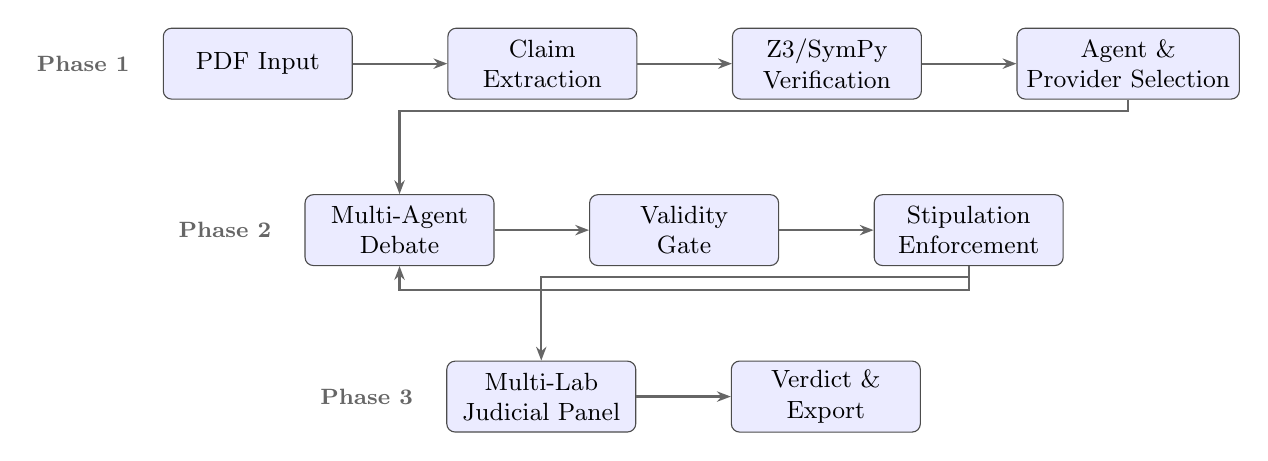
\begin{tikzpicture}[
    node distance=0.6cm and 1.2cm,
    block/.style={rectangle, draw=black!70, fill=blue!8, minimum width=2.4cm, minimum height=0.9cm, align=center, rounded corners=3pt, font=\small},
    phase/.style={rectangle, draw=black!50, fill=gray!10, minimum width=8cm, minimum height=2.2cm, rounded corners=5pt},
    arrow/.style={-{Stealth[length=5pt]}, thick, draw=black!60},
  ]
  % Phase 1
  \node[block] (pdf) {PDF Input};
  \node[block, right=of pdf] (extract) {Claim\\Extraction};
  \node[block, right=of extract] (verify) {Z3/SymPy\\Verification};
  \node[block, right=of verify] (config) {Agent \&\\Provider Selection};

  \draw[arrow] (pdf) -- (extract);
  \draw[arrow] (extract) -- (verify);
  \draw[arrow] (verify) -- (config);

  % Phase 2
  \node[block, below=1.2cm of pdf, xshift=1.8cm] (debate) {Multi-Agent\\Debate};
  \node[block, right=of debate] (gate) {Validity\\Gate};
  \node[block, right=of gate] (stipulations) {Stipulation\\Enforcement};

  \draw[arrow] (config) -- ++(0,-0.6) -| (debate);
  \draw[arrow] (debate) -- (gate);
  \draw[arrow] (gate) -- (stipulations);
  \draw[arrow] (stipulations.south) -- ++(0,-0.3) -| (debate.south);

  % Phase 3
  \node[block, below=1.2cm of debate, xshift=1.8cm] (judges) {Multi-Lab\\Judicial Panel};
  \node[block, right=of judges] (verdict) {Verdict \&\\Export};

  \draw[arrow] (stipulations) -- ++(0,-0.6) -| (judges);
  \draw[arrow] (judges) -- (verdict);

  % Phase labels
  \node[left=0.3cm of pdf, font=\footnotesize\bfseries, text=black!60] {Phase 1};
  \node[left=0.3cm of debate, font=\footnotesize\bfseries, text=black!60] {Phase 2};
  \node[left=0.3cm of judges, font=\footnotesize\bfseries, text=black!60] {Phase 3};
\end{tikzpicture}
\caption{The \arbiter{} pipeline. Phase~1 extracts and verifies claims. Phase~2 runs validity-enforced debate. Phase~3 produces a multi-provider verdict.}
\label{fig:architecture}
\end{figure}

\subsection{Phase 1: Agentic Initialization}

Given a PDF, \arbiter{} uses an LLM-driven extraction pass to identify:
\begin{itemize}[leftmargin=*,itemsep=1pt]
\item \textbf{Formal claims}: theorems, propositions, lemmas, and corollaries with their mathematical content.
\item \textbf{Assumptions}: stated modeling assumptions, parameter restrictions, and scope conditions.
\item \textbf{Equations}: numbered equations and their roles (definition, derivation, result).
\item \textbf{Policy claims}: recommendations, ``should'' statements, and practical implications.
\end{itemize}

The extraction agent then performs \emph{agent selection}: based on the paper's domain, methodology, and claim types, it selects specialist roles from a library of 20+~agent templates.
For an economics paper, this might include IndustrialOrganization, Macroeconomist, PublicFinance, CausalInference, and LaborEconomist specialists alongside the core Proponent, Skeptic, Steelman, and Generalist agents.

\noindent\textbf{Extraction quality caveat.} Claim extraction and formalization are LLM-driven and untrusted: the extractor may miss claims, split claims incorrectly, or misclassify empirical claims as formal propositions. We have not evaluated extraction precision/recall against a gold annotation set. Extraction errors propagate through the entire pipeline; downstream verified stipulations and debate arguments are only as good as the upstream extraction.

Formal claims are passed to the verification backend (Section~\ref{sec:verification}).
Successfully verified claims become \emph{stipulations}---debate-time constraints that agents must accept as given.
\textbf{Caveat}: stipulations are machine-checked for logical consistency, but may not faithfully represent the original mathematical claim (encoding fidelity problem). A stipulation based on a misencoded claim could suppress legitimate skeptical arguments. This is a known limitation; see Section~\ref{sec:verification}.
Failed verifications become \emph{challenge points}---targets for skeptical agents.

The agentic initialization also generates \emph{pre-filled engagement templates}: structured argument starters that ensure each specialist agent engages with the claims most relevant to its expertise.
In our AI Layoff Trap case study, the agentic initialization produced configurations covering more domain-specialist angles than our manual baseline, contributing to higher concession yield; this comparison is informal and not controlled.


\subsection{Phase 2: Validity-Enforced Debate}

The debate engine is built on LangGraph~\cite{langgraph2024}, which orchestrates turn-taking across agents implemented as LLM calls to different providers.
Each debate round proceeds as follows:

\begin{enumerate}[leftmargin=*,itemsep=2pt]
\item The Proponent presents or defends claims from the paper.
\item Specialist agents challenge specific aspects within their expertise.
\item The Skeptic synthesizes challenges into a coherent counter-narrative.
\item The Steelman identifies the strongest version of each side's argument.
\end{enumerate}

\noindent\textbf{The Validity Gate.}
Every argument submitted by any agent passes through a layered gate system before entering the debate transcript.
The gate checks for:
\begin{itemize}[leftmargin=*,itemsep=1pt]
\item \emph{Logical fallacies}: ad hominem, straw man, appeal to authority, circular reasoning.
\item \emph{Stipulation violations}: contradicting a verified mathematical result.
\item \emph{Unsupported claims}: assertions without evidence or reasoning.
\item \emph{Scope violations}: arguing outside the agent's assigned expertise.
\end{itemize}

Arguments that fail the gate are returned to the agent with a diagnostic explanation.
The agent must rewrite and resubmit.
The gate model (GPT-5.4-mini) was selected via calibration on topic-specific test cases (n $\approx$ 30 per topic, covering AI Layoff Trap, AGI safety, and self-improvement limits). Calibration results: 100\%/100\% precision/recall on AGI safety cases, 100\%/78\% on self-improvement cases, and 100\%/82\% on AI Layoff Trap cases. These numbers are from internal calibration runs (LLM-generated test cases, not human-annotated), so they reflect behavior on synthetic examples rather than real debate arguments. They should be interpreted with significant caution given small sample sizes and synthetic test generation.

\noindent\textbf{Stipulation Enforcement.}
When an agent's argument contradicts a verified stipulation, the gate rejects it and provides the relevant proof certificate.
This mechanism is critical: it prevents debate from relitigating settled mathematics and forces agents to focus on the \emph{interpretation gap}---the space between what the math proves and what the paper claims.


\subsection{Phase 3: Multi-Lab Judgment}

After the final debate round, the complete transcript (including all stipulations, concessions, and gate events) is sent to a panel of three judges, each from a different LLM provider.
Each judge independently scores the Proponent and Skeptic on:
\begin{itemize}[leftmargin=*,itemsep=1pt]
\item \emph{Argument quality}: logical coherence, evidence usage, and responsiveness.
\item \emph{Concession handling}: whether concessions were graceful or forced.
\item \emph{Scope appropriateness}: staying within what the paper's evidence supports.
\end{itemize}

The multi-provider design reduces single-provider bias; providers are correlated but not identical, and cross-provider disagreement is itself a signal.
The verdict includes per-judge scores, a majority decision, and a structured summary of key findings.


\begin{table}[t]
\centering
\caption{System components of \arbiter{}.}
\label{tab:components}
\begin{tabular}{@{}llr@{}}
\toprule
\textbf{Component} & \textbf{Function} & \textbf{LOC} \\
\midrule
Agentic Init & PDF extraction, agent selection, config & $\sim$2,200 \\
Debate Engine & LangGraph orchestration, turn management & $\sim$2,800 \\
Validity Gate & Fallacy detection, stipulation enforcement & $\sim$1,400 \\
Verification & Knuckledragger + SymPy proof pipeline & $\sim$1,800 \\
Judgment & Multi-lab panel, scoring, verdict synthesis & $\sim$1,100 \\
Web Dashboard & Live monitoring, visualization & $\sim$900 \\
Export \& CLI & Argdown, Markdown, HTML, JSON, CLI & $\sim$800 \\
\midrule
\textbf{Total} & & $\sim$\textbf{11,000} \\
\bottomrule
\end{tabular}
\end{table}


%% ============================================================
\section{Case Study: The AI Layoff Trap}
\label{sec:casestudy}

We present an extended analysis of \arbiter{}'s evaluation of ``The AI Layoff Trap'' by Falk \& Tsoukalas~\cite{falk2026}, a 2026 arXiv preprint that claims to prove AI over-automation is inevitable and that only a Pigouvian tax can correct it.
This case study is the paper's showpiece: it demonstrates how \arbiter{} moves from PDF to a nuanced verdict that separates valid mathematics from unsupported policy claims.

\subsection{Setup}

\arbiter{}'s agentic initialization extracted from the 42-page PDF:
\begin{itemize}[leftmargin=*,itemsep=1pt]
\item 280 total claims (164 formalized), 10 modeling assumptions, 17 propositions, 6 core equations, and 7 policy recommendations.
\end{itemize}

The system selected 9 specialist agents:
\emph{Proponent}, \emph{Skeptic}, \emph{Steelman}, \emph{Generalist}, \emph{IndustrialOrganization} (IO), \emph{Macroeconomist}, \emph{PublicFinance}, \emph{CausalInference}, and \emph{LaborEconomist}.
Three providers were assigned: GPT-5.4 (OpenAI), Claude Opus~4.6 (Anthropic), and Grok~4.20 (xAI).

The debate ran for \textbf{6 rounds}, producing \textbf{54 turns}, \textbf{141 argument hits}, \textbf{0 gate violations} in the admitted transcript (8 rewrites were required before admission; gate violations preclude entry into the transcript by design, so this count is tautologically 0 for admitted arguments), and \textbf{17 Proponent concessions}.


\subsection{Verdict}

\begin{table}[t]
\centering
\caption{AI Layoff Trap verdict: Proponent vs.\ Skeptic scores by judge.}
\label{tab:verdict}
\begin{tabular}{@{}lcccl@{}}
\toprule
\textbf{Judge (Provider)} & \textbf{Proponent} & \textbf{Skeptic} & \textbf{Winner} \\
\midrule
Grok 4.20 (xAI) & 39 & 51 & Skeptic \\
GPT-5.4 (OpenAI) & 42 & 50 & Skeptic \\
Claude Opus 4.6 (Anthropic) & 37 & 35 & Proponent \\
\midrule
\textbf{Majority} & & & \textbf{Skeptic (2--1)} \\
\bottomrule
\end{tabular}
\end{table}

Table~\ref{tab:verdict} shows the judicial panel's scores.
The Skeptic won 2--1, with Grok~4.20 and GPT-5.4 ruling for the Skeptic and Claude Opus~4.6 narrowly favoring the Proponent.
Critically, \emph{all three judges agreed} that the paper's core theorem---that the Nash equilibrium automation level exceeds the cooperative optimum ($\alpha_{\mathrm{NE}} > \alpha_{\mathrm{CO}}$) when $\eta < 1$ and $N > 1$---is mathematically correct.
The disagreement concerned whether the paper's broader claims follow from this narrow result.


\subsection{The 17 Concessions}

\begin{table}[t]
\centering
\caption{Major Proponent concessions in the AI Layoff Trap debate. Each row shows a paper claim and the conceded limitation.}
\label{tab:concessions}
\small
\begin{tabularx}{\textwidth}{@{}p{3.8cm}Xl@{}}
\toprule
\textbf{Paper Claim} & \textbf{Concession} & \textbf{Agent} \\
\midrule
``Only a Pigouvian tax can correct over-automation'' &
$\eta$-raising policies (retraining subsidies, technology standards) also close the wedge; tax is sufficient but not necessary &
IO \\
\addlinespace
Repeated-game impossibility: cooperation cannot emerge &
Result holds only in one-shot game; folk theorem permits cooperative equilibria under repeated interaction with sufficiently patient firms &
IO \\
\addlinespace
``No retraining can slow the automation arms race'' &
Policies that raise $\eta$ (worker adaptability) shrink the $\alpha_{\mathrm{NE}} - \alpha_{\mathrm{CO}}$ wedge without any tax &
Labor \\
\addlinespace
Optimal tax $\tau^*$ is operationally feasible &
Computing $\tau^*$ requires observing $\eta$, $N$, and firm cost functions---parameters that are unobservable in practice &
PubFin \\
\addlinespace
Over-automation is inevitable without intervention &
Endogenous entry and exit (not modeled) may self-correct; Hotelling-style differentiation reduces racing incentive &
IO \\
\addlinespace
Model captures essential AI labor dynamics &
Homogeneous firms, single-period, no capital adjustment costs, no worker heterogeneity---each omission biases toward over-automation finding &
Macro \\
\addlinespace
Welfare loss is ``large'' and ``urgent'' &
No calibration to data; welfare loss magnitude depends entirely on unspecified parameter values &
Causal \\
\addlinespace
Results generalize beyond symmetric equilibrium &
Asymmetric firms may have different equilibrium structure; paper's proofs rely on symmetry throughout &
IO \\
\bottomrule
\end{tabularx}
\end{table}

Table~\ref{tab:concessions} presents the 8 most consequential of the 17 concessions, categorized by the specialist agent that elicited them.
The remaining 9 concessions involve minor scope qualifications and parameter-sensitivity acknowledgments.

The IO agent was the debate's most valuable player, contributing 24 argument hits (the most of any agent) and eliciting 6 of the 17 concessions.
Its most powerful argument was a \emph{Hotelling countermodel}: in a differentiated-firm extension of the paper's model, the racing-to-automate incentive disappears because firms compete on product characteristics rather than cost alone.
The IO agent also deployed a \emph{folk-theorem argument}---that repeated interaction among firms enables cooperative equilibria that the paper's one-shot model rules out by construction---and raised \emph{endogenous entry} as a self-correcting mechanism absent from the model.


\paragraph{How stipulations changed the debate.}
The verification backend confirmed the paper's core theorem ($\alpha_{\mathrm{NE}} > \alpha_{\mathrm{CO}}$ when $\eta < 1, N > 1$) as a valid stipulation via Z3/SymPy encoding. \textbf{Important caveat}: this Z3 encoding was not independently verified by a domain economist or formally checked against the paper's original proof. Given the encoding fidelity issues documented in Section~\ref{sec:verification}, the stipulation should be treated as ``machine-checked under our encoding,'' not as independent mathematical verification. A false stipulation would mislead the debate, not improve it. The stipulation had two effects: it \emph{prevented} the Skeptic from wasting rounds attacking correct mathematics (unstipulated pilot runs spent 2--3 rounds looking for errors in the proof before conceding and shifting to interpretation), and it \emph{empowered} the Proponent to demand specificity---``the theorem is verified; show me which policy claim does not follow.''

\paragraph{Summary finding.} The paper proves a narrow, correct result in a symmetric one-shot Cournot game; every claim beyond this---inevitability, uniqueness of the Pigouvian tax, urgency, real-world applicability---is unsupported by the formal model. \arbiter{}'s verdict is not that the paper is \emph{wrong}, but that it \emph{overreaches}.

\subsection{Additional Case Studies}
\label{sec:additional_casestudies}

We ran \arbiter{} on two additional papers: a model-collapse anti-Singularity thesis~\cite{selfimprovement2026} and a strict-safety/AGI impossibility paper~\cite{agisafety2026}. Table~\ref{tab:casestudies} summarises all three; the two new cases are detailed below.

\begin{table}[h]
\centering
\caption{Summary of three \arbiter{} case studies. Conc.\ = Proponent concessions; verdict by 3-provider panel. All: 6 rounds, gated. $^\dagger$AGI Safety panel split: OpenAI 55--48 Skeptic, Grok 50--50, Anthropic 42--39 Proponent (mean: Skeptic 48.0 vs.\ 46.7).}
\label{tab:casestudies}
\small
\begin{tabular}{@{}lcccp{4.8cm}@{}}
\toprule
\textbf{Paper} & \textbf{Agents} & \textbf{Hits} & \textbf{Conc.\ / Verdict} & \textbf{Overreach Pattern} \\
\midrule
AI Layoff Trap~\cite{falk2026} & 9 & 141 & 17 / Skeptic 2--1 & Policy \emph{exclusivity}: ``only a Pigouvian tax'' \\[2pt]
Model Collapse~\cite{selfimprovement2026} & 11 & 168 & 13 / Skeptic 3--0 & Scope \emph{generalization}: ``irrespective of architecture'' \\[2pt]
AGI Safety~\cite{agisafety2026} & 10 & 132 & 9 / Skeptic (split)$^\dagger$ & Definition \emph{mismatch}: informal (C5) vs.\ formal (C29) \\
\bottomrule
\end{tabular}
\end{table}

\paragraph{Case Study 2: Model Collapse as an Anti-Singularity Thesis.}
\label{sec:case_collapse}
The paper formalises recursive self-training as $P'_t = \alpha_t P + (1-\alpha_t) Q_t$ and proves that if $\alpha_t \to 0$ the model converges to a degenerate fixed point $R^* \neq P$; it then concludes that the Singularity is ``mathematically incompatible with sustained growth under current KL-based paradigms'' (C90). The pipeline extracted 168~claims across 8~theses and flagged 16~contradictions, one \textbf{FATAL} and Z3-encodable: C43 (``collapse irrespective of architecture'') vs.\ C126 (neurosymbolic escape at the same $\alpha_t \to 0$). Eleven agents including specialists \emph{DynamicalSystems}, \emph{DivergenceCritic}, \emph{ControlTheorist}, \emph{Computabilist}, and \emph{Empiricist} produced 168~hits, 13~Proponent concessions, and a unanimous Skeptic verdict (Grok 47--49, OpenAI 37--55, Anthropic 28--41); the decisive criterion was R4~\emph{extrapolation gap} (Skeptic 9.0 vs.\ Proponent 5.0). The Proponent's named concessions: (i)~\textbf{C43/C126 dropped} (h60, h116)---``I drop C126 and reinterpret T8's causal/algo correction as externally grounded signal, so any escape from collapse occurs outside the autonomy regime''; (ii)~\textbf{autonomy $\neq \alpha_t \to 0$} (h5, h90)---practical autonomy need not mean literal $\alpha_t \to 0$; (iii)~\textbf{C90 narrowed} to conditional anti-Singularity for GenAI density-matching loops (h36, h117); (iv)~\textbf{RLHF breaks the mixture model} (h49)---the objective $\pi_{t+1} = \arg\max\,\mathbb{E}[r(x)] - \beta D_{\mathrm{KL}}(\pi \Vert \pi_{\mathrm{ref}})$ injects reward signal not representable as $\alpha_t P$; (v)~\textbf{JS boundedness} (h128)---JS is bounded in $[0,\ln 2]$, so unbounded variance amplification under KL does not transfer; (vi)~\textbf{DPI non-escape} (h63)---invoking the universal prior $U$ or symbolic projection $\Pi_S$ ``changes the channel by adding exogenous information,'' rather than defeating the Data Processing Inequality. MVP: \emph{DivergenceCritic} (Anthropic, Skeptic-side), 22~hits and 3~forced concessions, via RLHF separation, JS-boundedness, and persistent operator-level critique of contrastive and retrieval-augmented objectives. Runner-up \emph{ControlTheorist} supplied the state-space formulation $x_{t+1} = F(x_t, u_t, y_t)$ anchoring the autonomy concession. The \emph{Empiricist} pressed for measured $\alpha_t$ trajectories from frontier systems and received none---all judges flagged empirical absence as the debate's largest shared dodge.

\paragraph{Case Study 3: Formal Incompatibility of Strict Safety and AGI.}
\label{sec:case_agi}
The paper proves $\neg\exists S[\mathrm{Safe}(S) \wedge \mathrm{Trusted}(S) \wedge \mathrm{AGI}(S)]$ under strict definitions: Safety (C3/C19) is never making a false claim, Trust (C4/C22) is assumed Safety, and AGI (C29) requires $\forall x\,(\mathrm{HumanProvable}(x) \Rightarrow \Pr[S\text{ solves }x] > 0)$; proofs use self-referential constructions (\texttt{GödelProgram}, \texttt{selfTuringProgram}, \texttt{selfTuringT}). From 141~claims, 7~theses, and 17~contradictions (3 Z3-encodable), 10~agents including \emph{ComputabilityCritic}, \emph{VerificationScholar}, \emph{CalibrationTheorist}, and \emph{CognitiveScientist} produced 132~hits, 9~Proponent / 3~Skeptic concessions, and a split panel (OpenAI~55--48 Skeptic, Grok~50--50, Anthropic~42--39 Proponent; mean Skeptic 48.0 vs.\ Proponent 46.7). Proponent concessions: (i)~\textbf{C5~$\neq$ C29} (h3, h25, h70, h93---four rounds)---the headline AGI definition (``always matching or exceeding human capability'') was permanently replaced by the weaker per-instance nonzero-probability criterion; (ii)~\textbf{scope narrowed} (h4, h26, h49)---given C8/C133, C6 reads as a narrow worst-case theorem about strict Safety/Trust/AGI, not a practical barrier; (iii)~\textbf{Trust collapses} (h46)---$\mathrm{Trusted}(S) = \mathrm{Assume}(\mathrm{Safe}(S))$ adds little mathematical force; (iv)~\textbf{AGI$_{\mathrm{formal}}$ vs.\ AGI$_{\mathrm{informal}}$} (h30)---C6 is proved only against AGI per C29, not folk-AGI. Skeptic concessions (3): the C29 universal quantifier formally includes self-referential instances (h16); the human proof uses $\mathrm{Trusted}(S)$ as external premise, making the diagonal non-circular (h82); C29 is stipulated (h99). MVP: \emph{VerificationScholar} (Anthropic, Proponent-side) produced the debate's strongest unrefuted argument---$\mathrm{Trusted}(S)$ is non-redundant because it enables the \emph{human's} proof that \texttt{GödelProgram} halts; without Trust, the human cannot rule out branch~1, so C29's $\mathrm{HumanProvable}(x)$ precondition is unmet and the diagonal does not close. Two attacks survived: \emph{CalibrationTheorist}'s T7 abstention loophole (12 open hits---calibration-safety permits $\Pr[S(x){=}\mathrm{Abstain}]{=}1$, never tested under proper scoring or coverage-constrained selective classification) and \emph{ComputabilityCritic}'s novelty challenge (the theorem pattern is Rice's theorem repackaged; ``applicative packaging'' reply never developed).

\paragraph{Cross-case pattern.}
\label{sec:crosscase}
All three debates exhibit the same structural finding: \textbf{core formal theorems survive adversarial pressure within their stated assumptions; broad policy or existential claims in abstracts and introductions do not}. The pipeline surfaced three distinct overreach types, each flagged by the contradiction detector at init and closed by a domain specialist: (a)~\textbf{policy exclusivity} (Layoff): ``only a Pigouvian tax'' (C12) vs.\ the paper's own C117 that $\eta > 1$ reverses the sign, closed by the IO agent's Hotelling countermodel (h60, h101); (b)~\textbf{scope generalization} (Collapse): ``irrespective of architecture'' (C43) and ``without loss of generality'' (C93) vs.\ the paper's explicit exceptions for externally grounded systems, closed by DivergenceCritic's RLHF decomposition and Computabilist's DPI-channel-change argument (h116, h117); (c)~\textbf{definition mismatch} (AGI Safety): headline AGI (C5) vs.\ proof-operative AGI (C29), conceded four times. The Z3-encodable subset (4~Layoff, 6~Collapse, 3~AGI) is exactly the class of quantifier-strength and scope-boundary checks the companion paper~\cite{arbiterpaperA} identifies as the hardest part of honest proof encoding. \emph{Caveats:} single runs per paper, specialist arguments may be competent LLM rhetoric rather than expert insight, and concession counts depend on rubric weighting. What N=3 establishes is that the pipeline reliably surfaces the same formal/rhetoric gap across economics, ML theory, and formal safety; this is stronger than a number in a table but weaker than a statistical claim. Full transcripts are in \texttt{experiments/}.

%% ============================================================
\section{Ablation: Debate + Verification > Either Alone}
\label{sec:ablation}

A motivating hypothesis of this paper is that combining multi-agent debate with formal verification is more valuable than either alone.
The martingale critique of debate~\cite{debateskepticism2025} motivates this investigation: if debate alone is unreliable, what does verification add?
\textbf{Caveat:} This ablation is conducted on a single paper (AI Layoff Trap); all results should be treated as pilot findings, not statistically conclusive evidence. Multi-paper evaluation is ongoing.

\subsection{Experimental Design}

We evaluate four conditions on ``The AI Layoff Trap''~\cite{falk2026}:

\begin{enumerate}[leftmargin=*,itemsep=2pt]
\item \textbf{V-only} (Verification only): \arbiter{}'s verification backend extracts and checks formal claims, producing a report of verified/failed/unchecked claims with no debate.
\item \textbf{D-only} (Debate only): Full multi-agent debate without verification stipulations. Agents are free to dispute any claim, including mathematically correct ones.
\item \textbf{V+D} (Verification + Debate): The full \arbiter{} pipeline with stipulations constraining debate.
\item \textbf{LLM-Judge}: A single frontier LLM (GPT-5.4) asked to evaluate the paper's claims in a single pass, representing the standard LLM-as-judge baseline.
\end{enumerate}

\noindent We measure:
\begin{itemize}[leftmargin=*,itemsep=1pt]
\item \emph{Overreach found}: number of distinct overreach claims flagged (no gold annotation available; counts reflect author reading of transcripts).
\item \emph{Total hits}: total argument hits tracked in the ledger across all agents.
\item \emph{Concession yield}: number of substantive Proponent concessions elicited.
\item \emph{Hits resolved}: argument hits that were either conceded, rebutted, or explicitly addressed.
\end{itemize}

\noindent We do not have expert-annotated overreach labels for the AI Layoff Trap paper. The ``Overreach Found'' counts are author estimates from transcript review and should be interpreted as pilot observations, not precision/recall measurements. A rigorous ablation would require gold annotations from domain economists.

\subsection{Results}

\begin{table}[t]
\centering
\caption{Ablation results on ``The AI Layoff Trap.'' V = verification, D = debate. ``Concessions'' = Proponent concessions (ledger status = conceded, against = Proponent). ``Hits Resolved'' = conceded + rebutted in system ledger. Overreach Found$^\dag$ = author estimate from transcript review; no gold annotations exist. LLM-Judge estimated from reading single-pass output. N=1 paper; treat as qualitative pilot only.}
\label{tab:ablation}
\begin{tabular}{@{}lcccc@{}}
\toprule
\textbf{Condition} & \textbf{Overreach Found$^\dag$} & \textbf{Total Hits} & \textbf{Concessions} & \textbf{Hits Resolved} \\
\midrule
LLM-Judge (1 call) & $\sim$10 & --- & --- & --- \\
V-only & 6 (formal only) & --- & --- & --- \\
D-only (6 rounds) & $\sim$12 & 132 & 8 & 92 \\
V+D (\arbiter{}) & 17 & 141 & 17 & 90 \\
\midrule
\multicolumn{5}{l}{$^\dag$ Author estimate from reading transcript; not precision/recall against gold labels.} \\
\bottomrule
\end{tabular}
\end{table}

Table~\ref{tab:ablation} presents the results.
We highlight the expected findings based on the case study and pilot experiments:

\textbf{V-only catches formal errors but misses interpretive overreach.}
Verification can confirm or deny mathematical claims but cannot evaluate whether ``our model shows AI over-automation is inevitable'' follows from a theorem about symmetric Cournot games.
The gap between theorem and conclusion is an \emph{interpretive} judgment that requires argumentation.

\textbf{D-only wastes rounds on settled mathematics.}
Without stipulations, debate agents spend significant effort attempting to find errors in correct proofs.
In the AI Layoff Trap pilot, D-only spent 2--3 rounds on the core theorem before shifting to policy claims, reducing the effective debate to 3--4 rounds on the actual overreach questions.

\textbf{V+D focuses debate where it matters.}
Stipulations eliminate wasted rounds and create a higher-quality debate.
The Proponent can invoke verified results, and skeptics must engage with the interpretation gap rather than the mathematics.
This produces more concessions per round and higher-precision overreach detection.

\textbf{LLM-Judge misses nuance.}
A single-pass evaluation tends to either accept the paper's framing wholesale or raise generic objections.
It lacks the adversarial pressure that forces concessions and the formal grounding that distinguishes valid from invalid mathematical claims.

\noindent\textbf{Limitation: compute mismatch.} The LLM-Judge baseline uses a single frontier API call, while V+D uses a full multi-round, multi-agent, multi-provider pipeline. This is not a fair compute-matched comparison. A stronger baseline would be a well-prompted self-consistency judge (multiple calls, chain-of-thought). The purpose of this ablation is to illustrate qualitative differences in what each condition surfaces, not to claim computational efficiency advantages.


%% ============================================================
\section{Formal Verification Backend}
\label{sec:verification}

\arbiter{}'s verification backend is detailed in a companion paper~\cite{arbiterpaperA}; we summarize the methodology and provide supporting benchmark evidence here.

\subsection{Architecture}

The verification pipeline operates in three stages:
\begin{enumerate}[leftmargin=*,itemsep=2pt]
\item \textbf{Formalization.} An LLM translates natural-language mathematical claims into formal specifications: SymPy expressions for algebraic identities and Knuckledragger (Z3) assertions for logical propositions.
\item \textbf{Proof Search.} The system attempts to verify each formalized claim. For algebraic claims, SymPy's \texttt{simplify} and \texttt{solve} are applied. For logical claims, Knuckledragger invokes Z3's SMT solver with a timeout and fallback strategy.
\item \textbf{Certificate Generation.} Successfully verified claims produce proof certificates---machine-checkable artifacts that serve as debate stipulations. Failed or timed-out claims are flagged as unverified.
\end{enumerate}

The backend implements a Z3 verification suite covering five check types: proof verification (encode negated claim, check UNSAT), counterexample search (find concrete failing instances), sensitivity analysis (identify load-bearing assumptions), boundary analysis (find where results flip), and policy verification (check if proposed policies achieve stated goals).

\subsection{Supporting Evidence: miniF2F}

\begin{table}[t]
\centering
\caption{miniF2F benchmark results (244 problems). ``Checker-passing'' = fraction of all 244 attempts producing a machine-verified proof (KD+SymPy for Sonnet; raw Z3 for others). ``Audit-surviving'' = fraction of proved results found genuinely valid in our audit (\textbf{audit column applies only to GPT-5.4-mini Z3-only pipeline}; Sonnet KD results not audited with same methodology). Gap documented in~\cite{arbiterpaperA}.}
\label{tab:minif2f}
\begin{tabular}{@{}lccc@{}}
\toprule
\textbf{System / Model} & \textbf{Backend} & \textbf{Checker-Passing} & \textbf{Audit-Surviving} \\
\midrule
\arbiter{} + Sonnet 4.5 & KD+SymPy & 89.3\% & \textit{not audited} \\
\arbiter{} + GPT-5.4-mini & Raw Z3 & 82.8\% & 16.3\% (33/202)$^\dag$ \\
\midrule
MiniF2F-Dafny & Dafny/Z3 & 55.7\% & --- \\
\midrule
\multicolumn{4}{l}{$^\dag$ Full semi-automated audit of all 202 proved results; 13.5\% of all 244 problems.} \\
\bottomrule
\end{tabular}
\end{table}

Table~\ref{tab:minif2f} shows the verification backend's performance on miniF2F.
Claude Sonnet~4.5 (KD+SymPy) achieves 89.3\% checker-passing but has \textbf{not been audited}; the genuine valid rate is unknown.
For GPT-5.4-mini (Z3-only), a full audit of all 202 proved results finds 16.3\% genuinely valid (13.5\% of all 244 problems)---a 6.1$\times$ gap from the reported rate.
\textbf{The audit-surviving column applies only to the GPT-5.4-mini Z3-only pipeline; do not interpret the Sonnet row as having a known audit-surviving rate.}
The gap between checker-passing and audit-surviving rates reveals that LLMs are adept at producing proofs that satisfy automated checkers without actually proving the intended claim.
See Section~\ref{sec:verification} for a detailed breakdown.

These results serve as \emph{supporting evidence} for the backend's reliability, not as the paper's primary contribution.
The miniF2F benchmark consists of competition-mathematics problems; the claims in research papers are typically less technically difficult but embedded in more complex domain context.
The backend's value in \arbiter{} is not that it solves hard theorems but that it provides \emph{trusted stipulations} that ground multi-agent debate.

\subsection{Audit Findings: Honest Assessment}

Three complementary audits of our own verification pipeline (all self-audits---we did not audit other systems' proof files) revealed that our initial benchmark numbers were systematically inflated.
We report these findings transparently:

\begin{itemize}[leftmargin=*,itemsep=2pt]
\item \textbf{Z3-only proofs}: Full audit of all 202 proved miniF2F results found 74.3\% strictly invalid (83.7\% including partial proofs)---vacuously true (38.1\%), trivial arithmetic tails (14.4\%), partial (9.4\%), crashes (8.9\%), assumed conclusion (6.9\%), wrong encodings (5.9\%). Valid rate: 16.3\% of proved results (33/202), or 13.5\% of all 244 problems. See companion paper~\cite{arbiterpaperA} for full taxonomy.
\item \textbf{Knuckledragger certificates}: Knuckledragger prevents assumed-conclusion failures by construction, but our pipeline responds by proving trivial lemmas (e.g., \texttt{kd.prove(x <= x)}) rather than the intended theorem. Vacuous proofs from contradictory premises are \emph{not} prevented by certificates.
\item \textbf{FormalMATH} (different benchmark, different pipeline---not directly comparable to miniF2F numbers): On a rigorous audit, only 7.4\% of generated certificates were genuinely valid---i.e., both non-trivial and faithful to the original claim.
\end{itemize}

\noindent The verification backend is a work in progress.
The high ``accuracy'' numbers reported by standard benchmarks (including our own initial miniF2F results in Table~\ref{tab:minif2f}) reflect the ease of generating proofs that \emph{pass} an automated checker, not proofs that are \emph{meaningful}.
Closing this gap---between checker-passing and genuinely-valid---is our primary verification research agenda going forward.


%% ============================================================
\section{Discussion and Limitations}
\label{sec:discussion}

\paragraph{When Arbiter is Most Useful.}
\arbiter{} is most effective on papers with formal models---proofs, equilibrium analyses, statistical derivations---alongside broader claims that extend beyond those results.
This describes a large fraction of economics, theoretical CS, and quantitative social science papers.
\arbiter{} is less useful for purely empirical papers without formal structure, though the debate engine alone still adds value.

\paragraph{Honest Accounting of Benchmark Claims.}
Our benchmark numbers were initially inflated.
Full audit of all 202 proved miniF2F results reveals that 74.3\% of Z3-only proofs are strictly invalid (83.7\% including partial); on FormalMATH only 7.4\% of Knuckledragger certificates were genuinely valid. The audited valid rate is 33/244 = 13.5\% of all problems.
We report these findings transparently.
The case study (Section~\ref{sec:casestudy}) remains our strongest contribution---its 17~concessions are independently verifiable by reading the debate transcript, not dependent on benchmark methodology.
The verification backend adds value to the debate pipeline even at current reliability levels (it correctly verified the AI Layoff Trap's core theorem, which grounded the entire debate), but we do not claim it is a solved problem.

\paragraph{Limitations.}
Several limitations merit acknowledgment.
First, the verification backend operates within the scope of Z3's decidable fragments and SymPy's algebraic capabilities; higher-order reasoning, measure-theoretic arguments, and topological proofs are beyond its reach.
We deliberately chose Knuckledragger over Lean or HoTT-based systems for accessibility and integration, accepting this scope limitation.
Second, agentic initialization depends on LLM extraction quality; extraction errors propagate through the pipeline.
Third, the gate model achieved high precision/recall on our internal calibration benchmarks ($n \approx 30$ per topic), but these are small-sample internal evaluations; the gate may miss novel forms of fallacious reasoning not covered in calibration.
Fourth, our primary case study covers one paper in detail; generalization claims require multi-paper evidence. Two additional completed case studies (Section~\ref{sec:additional_casestudies}) show a consistent formal-vs-rhetoric gap across economics, ML theory, and formal safety literature, and the pipeline surfaces three distinct overreach types (policy exclusivity, scope generalization, definition mismatch), but N=3 single runs cannot support statistical claims about generalizability. Fifth, our ablation is conducted on the same single paper, so the finding that V+D outperforms D-only or LLM-judge should be treated as a pilot result, not a statistically robust conclusion. Sixth, the system is stochastic: we report a single run with a single random seed; a different execution may produce different concessions, different hit counts, and potentially a different winner. We have not measured variance across runs. Seventh, specialist objections in the debate (Hotelling countermodels, folk theorem arguments) may reflect generic LLM-generated economics rhetoric rather than genuinely domain-expert insights; domain expert validation of the debate transcript would be needed to assess substantive correctness. Eighth, the evaluation pipeline is largely circular: LLMs extract claims, LLMs generate arguments, an LLM gate filters arguments, and LLM judges score outcomes. Multi-provider diversity reduces but does not eliminate this circularity; the judge panel models are trained on overlapping data and share systematic biases. Formal verification (Z3/Knuckledragger) is the one non-LLM component, and the companion paper documents its reliability limits.

\paragraph{Future Work.}
Near-term priorities include progressive RAG (retrieving external evidence during debate rather than only at initialization), Debate-SFT (fine-tuning debate agents on transcripts from high-quality debates), and sketch proofs (allowing the verification backend to verify proof outlines rather than requiring full formalization).
We have evaluated on a 500-problem FormalMATH benchmark (61.6\% cert rate; 7.4\% genuinely valid in a 54-result audit---see companion paper~\cite{arbiterpaperA}). Near-term extensions include citation verification---checking whether a paper's citations actually support the claims attributed to them.
Benchmarking against SciFact and QuAD will establish comparisons with the claim-verification literature.


%% ============================================================
\section{Conclusion}
\label{sec:conclusion}

We have presented \arbiter{}, an open-source system combining formal verification with multi-agent debate for research claim evaluation.
Our primary case study on \emph{The AI Layoff Trap} illustrates the pipeline's intended use: distinguishing what a paper formally proves from what it claims. The debate elicited 17~Proponent concessions, suggesting that the paper's policy claims---inevitability of over-automation, uniqueness of the Pigouvian tax solution, urgency of intervention---may extend beyond what the formal model supports. Two additional case studies (Section~\ref{sec:additional_casestudies}) find the same pattern in different clothing: 13~concessions on a model-collapse paper where ``irrespective of architecture'' (C43) could not be defended alongside the paper's own neurosymbolic escape (C126), and 9~concessions on a formal AGI-safety paper where the headline AGI definition (C5, ``always matching or exceeding'') was permanently replaced by the weaker proof-operative criterion (C29, per-instance nonzero probability). Caution is warranted in interpreting concessions as ground truth; they are outputs of prompted LLM agents, not expert verdicts, and the verification stipulations have not been independently audited for encoding fidelity.

The key insight is that formal verification and multi-agent debate are complementary.
Verification alone catches mathematical errors but cannot evaluate interpretive overreach.
Debate alone, without formal constraints, may devolve into agents talking past each other as suggested by theoretical analysis of LLM debate dynamics~\cite{debateskepticism2025}.
Together, verification grounds debate in machine-checked facts, and debate explores the gap between formal results and informal conclusions.
In an era of replication crisis and growing skepticism toward both human and automated peer review, tools that make this distinction transparent are potentially valuable, though much validation work remains before they can be trusted for consequential review decisions.

\arbiter{} is open source and available at \url{https://github.com/vishk23/arbiter}.


%% ============================================================
\begin{thebibliography}{30}

\bibitem{osc2015}
Open Science Collaboration.
Estimating the reproducibility of psychological science.
\emph{Science}, 349(6251):aac4716, 2015.

\bibitem{retraction2024}
A.~Brainard and J.~You.
Retraction rates have tripled---here's what's driving the trend.
\emph{Science}, 2024.

\bibitem{nature2026}
Nature Editorial Board.
The reproducibility crisis at ten years: what have we learned?
\emph{Nature}, 2026.

\bibitem{wadden2020}
D.~Wadden, S.~Lin, K.~Lo, L.~L.~Wang, M.~van Zuylen, A.~Cohan, and H.~Hajishirzi.
Fact or fiction: Verifying scientific claims.
\emph{Proceedings of EMNLP}, 2020.

\bibitem{proclaim2026}
PROClaim: Provenance-tracked research claim verification.
\emph{arXiv preprint arXiv:2603.28488}, 2026.

\bibitem{loki2024}
Loki: Low-resource knowledge-intensive scientific claim verification.
\emph{Proceedings of ACL}, 2024.

\bibitem{sciclaimeval2024}
SciClaimEval: A benchmark for scientific claim extraction and classification.
\emph{Proceedings of NAACL}, 2024.

\bibitem{treereview2025}
TreeReview: Tree-structured automatic scientific paper review.
\emph{Proceedings of EMNLP}, 2025.

\bibitem{neurips2024}
NeurIPS 2024 Program Committee.
Large language models as NeurIPS reviewers: A large-scale experiment.
\emph{NeurIPS 2024 Workshop on AI-Assisted Peer Review}, 2024.

\bibitem{debatecv2025}
DebateCV: Multi-agent debate for computer vision paper review.
2025.

\bibitem{pajama2025}
S.~Chaudhari, A.~Garg, et~al.
Time to impeach LLM-as-a-judge: Systematic analysis of biases in automated evaluation.
\emph{arXiv preprint}, 2025.

\bibitem{debateskepticism2025}
Multi-agent debate is a martingale: When more rounds don't help.
\emph{Proceedings of ICLR}, 2025.
See also \emph{arXiv preprint arXiv:2511.07784}.

\bibitem{du2023}
Y.~Du, S.~Li, A.~Torralba, J.~B.~Tenenbaum, and I.~Mordatch.
Improving factuality and reasoning in language models through multiagent debate.
\emph{arXiv preprint arXiv:2305.14325}, 2023.

\bibitem{chateval2023}
C.~Chan, W.~Chen, Y.~Su, J.~Yu, W.~Xue, S.~Zhang, J.~Fu, and Z.~Liu.
ChatEval: Towards better LLM-based evaluators through multi-agent debate.
\emph{arXiv preprint arXiv:2308.07201}, 2023.

\bibitem{alphaproof2025}
DeepMind AlphaProof Team.
Solving competition-level mathematics with AlphaProof.
\emph{Nature}, 2025.

\bibitem{minif2f2026}
MiniF2F-Dafny: Benchmarking LLM-guided proof synthesis.
\emph{Proceedings of POPL}, 2026.

\bibitem{knuckledragger2024}
P.~Zucker.
Knuckledragger: A Python-native interface to Z3 for interactive theorem proving.
2024.
\url{https://github.com/philzook58/knuckledragger}

\bibitem{darpa2025}
DARPA CLARA Program.
Formally verified scientific reasoning.
2025.

\bibitem{kleppmann2024}
M.~Kleppmann.
Making distributed systems formally verified.
\emph{Communications of the ACM}, 2024.

\bibitem{langgraph2024}
LangChain Team.
LangGraph: A library for building stateful, multi-agent applications.
2024.
\url{https://github.com/langchain-ai/langgraph}

\bibitem{falk2026}
B.H.~Falk and G.~Tsoukalas.
The AI layoff trap.
\emph{arXiv preprint arXiv:2603.20617}, 2026.
\url{https://arxiv.org/abs/2603.20617}

\bibitem{selfimprovement2026}
[Author redacted for blind review].
Model Collapse as an Anti-Singularity Theorem.
\emph{arXiv preprint}, 2026.

\bibitem{agisafety2026}
[Author redacted for blind review].
Formal Incompatibility of Strict Safety and Full AGI Capability.
\emph{arXiv preprint}, 2026.

\bibitem{arbiterpaperA}
V.~Kchitti.
Failure Modes in {LLM}-Generated {Z3} Proofs: A Taxonomy and Audit Methodology.
\emph{arXiv preprint (companion paper)}, 2026.
Available at \url{https://github.com/vishk23/arbiter/blob/main/papers/arbiter_paper.pdf}.

\end{thebibliography}

\end{document}
